\NoBgThispage
\chapter{Analysis of Results and Future Improvements}

This chapter presents a comparison of the results obtained from the two approaches investigated in this work. The strengths and limitations of each approach will be analyzed, and their potential real-world applications will be discussed. Additionally, future developments and improvements to enhance the performance and applicability of the methods will be proposed.

\section{Achievements and Real-World Applications}

As detailed in Chapter 3, the two approaches investigated exhibited distinctly different behaviors. The first approach, while conceptually simple, proved to be impractical for implementation based on the evaluation results. Even in the best-case scenarios, the accuracy achieved by this method was insufficient to make it a standalone localization solution for ground truth generation. When compared to state-of-the-art techniques, the performance of this method was analogous to classical localization methods from the late 2000s that did not utilize sensor fusion.

This first approach could potentially be integrated into a pipeline that minimizes point-segment distances iteratively, where a human operator initially fixes key points. Such a pipeline could automate the process of removing the need for human intervention but would still require iterative optimization. An example of this proposed pipeline is shown in Figure~\ref{fig:mapalign_optimizer}.

\begin{figure}[H]
    \centering
    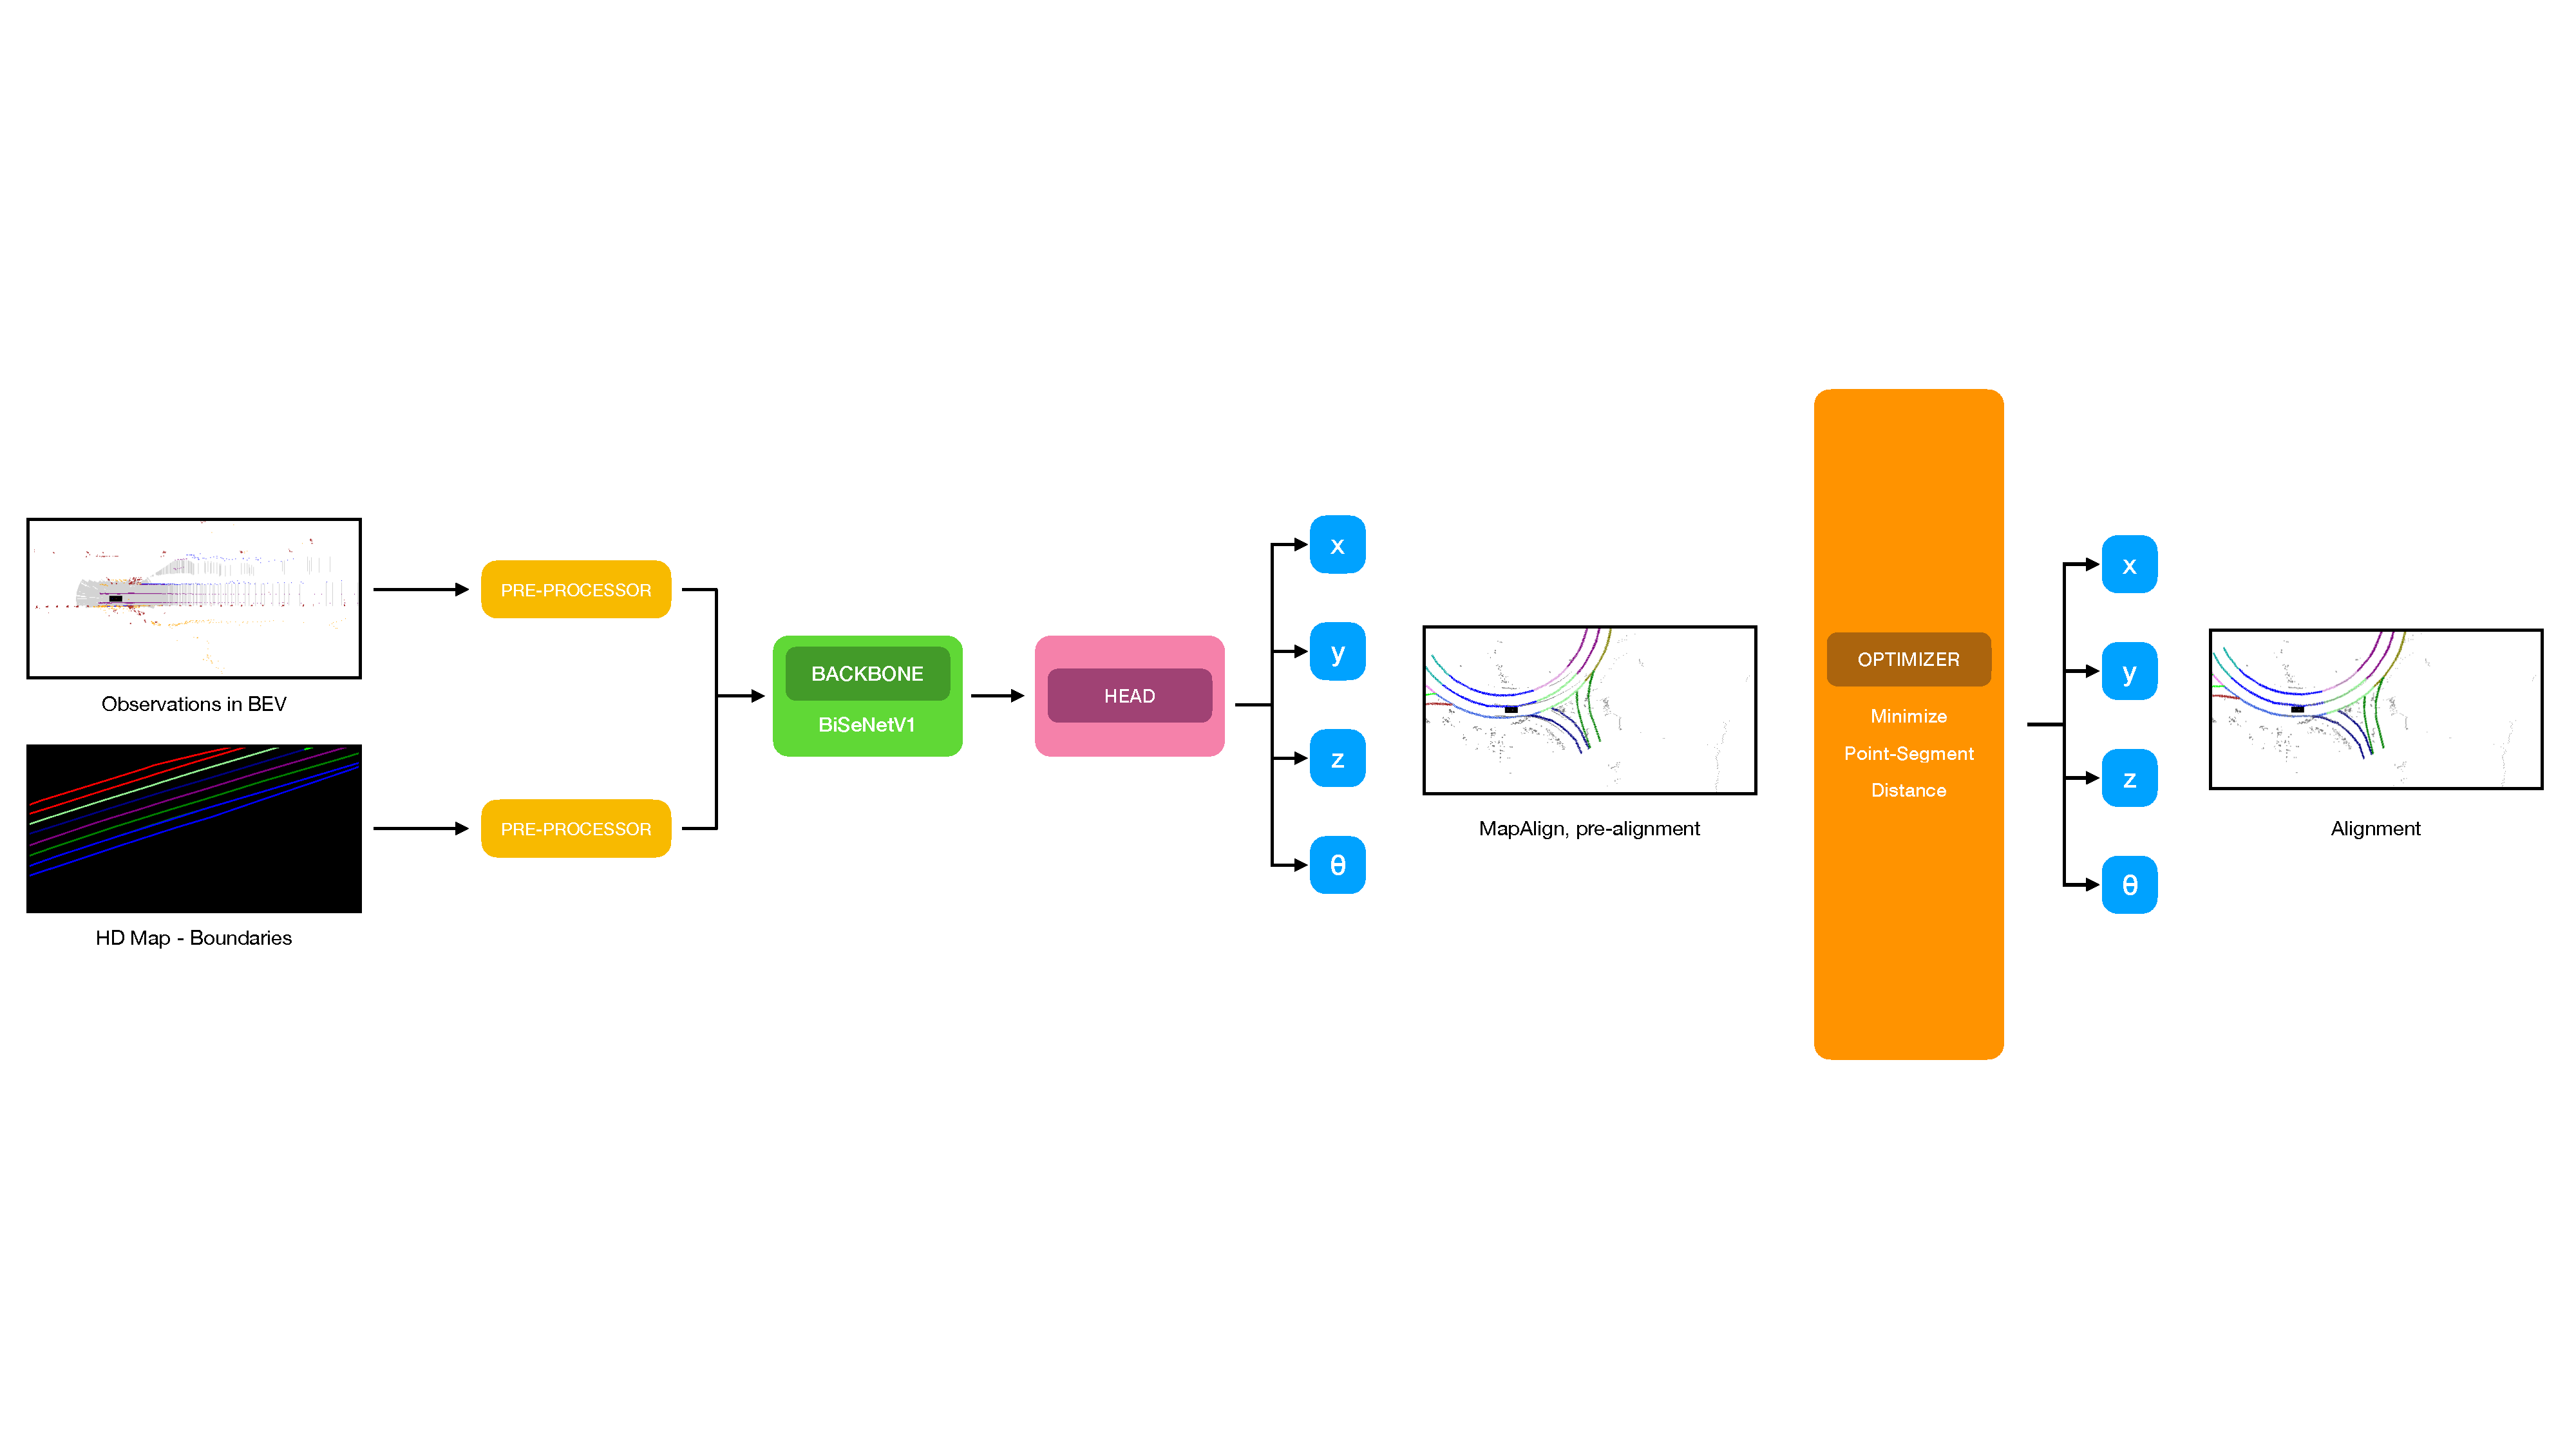
\includegraphics[width=1\linewidth]{LateX//figs/mapalign_optimizer.pdf}
    \caption{Proposed pipeline for integrating the first approach into an iterative optimization workflow.}
    \label{fig:mapalign_optimizer}
\end{figure}

The second approach, incorporating bird’s-eye view (BEV) reconstruction, demonstrated significant improvements over the first and surpassed the capabilities defined by the state of the art, at least within the dataset used for training and testing. While this approach requires an advanced and costly sensor suite, its redundancy in sensor usage could be reduced to make the system more cost-effective without compromising performance.

Table~\ref{tab:evaluation_results_2} summarizes all the attempts made, highlighting the best results for each architecture in bold. The table provides a clear comparison of the methods and the effectiveness of the proposed approaches.


\begin{table}[H]
\centering
\caption{Evaluation Results}
\label{tab:evaluation_results_2}
\scriptsize % Adjust font size for compactness
\renewcommand{\arraystretch}{1} % Add a bit of padding between rows for readability
\begin{tabular}{llcllccr}
\toprule
\textbf{Method} & \textbf{Dataset Split} & \makecell{\textbf{Heading}\\\textbf{Measurement}\\\textbf{Unit}} & \textbf{Batch Size} & \makecell{\textbf{Loss}\\\textbf{Function}} & \textbf{Iterations} & \makecell{\textbf{Eval}\\$\Delta$ \textbf{Pose}} & \makecell{\textbf{Eval}\\$\Delta \theta$} \\
\midrule
Just detector & Via Lang & RAD & 64 & MSE        & 100,000 & 1.54 & 1.15 \\
Just detector & Via Lang & RAD & 64 & L1         & 100,000 & 1.40 & 1.72 \\
Just detector & Via Lang & RAD & 64 & L1 Smooth  & 100,000 & 1.38 & 1.15 \\
Just detector & Via Lang & DEG & 64 & MSE        & 100,000 & 2.51 & 1.81 \\
Just detector & Via Lang & DEG & 64 & L1         & 100,000 & 2.05 & 1.45 \\
Just detector & Via Lang & DEG & 64 & L1 Smooth  & 100,000 & 1.65 & 1.10 \\
Just detector & All      & DEG & 64 & L1 Smooth  & 100,000 & 1.61 & 0.74 \\
BEV           & All      & DEG & 32 & L1 Smooth  & 100,000 & 0.01 & 0.004 \\
BEV           & All      & DEG & 32 & L1 Smooth  & 100,000 & 0.01 & 0.004 \\
\bottomrule
\end{tabular}
\end{table}



The potential real-world applications of these methods are promising. The second approach, in particular, could be employed for ground truth generation during dataset creation, as described in Chapter 1. This application focuses on generating high-definition (HD) maps in real time using the car’s sensor suite and a basic standard-definition (SD) map. As mentioned earlier, perfect alignment is critical for defining the input and target data of the network.

Furthermore, this method could be extended to enable online localization for autonomous vehicles using HD maps. However, this application would require the HD maps to be stored and maintained onboard the vehicle, bringing challenges such as storage limitations and associated costs, as discussed in previous chapters. Another limitation, not yet investigated in this work, is the latency introduced by the proposed system, which could impact real-time performance.


\section{Future Developments and Improvements}

An important direction for future work involves addressing the granularity of the grid, which is currently set at $25$ cm per pixel. While this precision is sufficient for the tasks performed in this study, it does not align with the centimeter-level precision typically associated with high-definition (HD) maps. One potential improvement, as illustrated in Figure~\ref{fig:grid}, involves incorporating additional spatial information into the input tensor.

\begin{figure}[H]
    \centering
    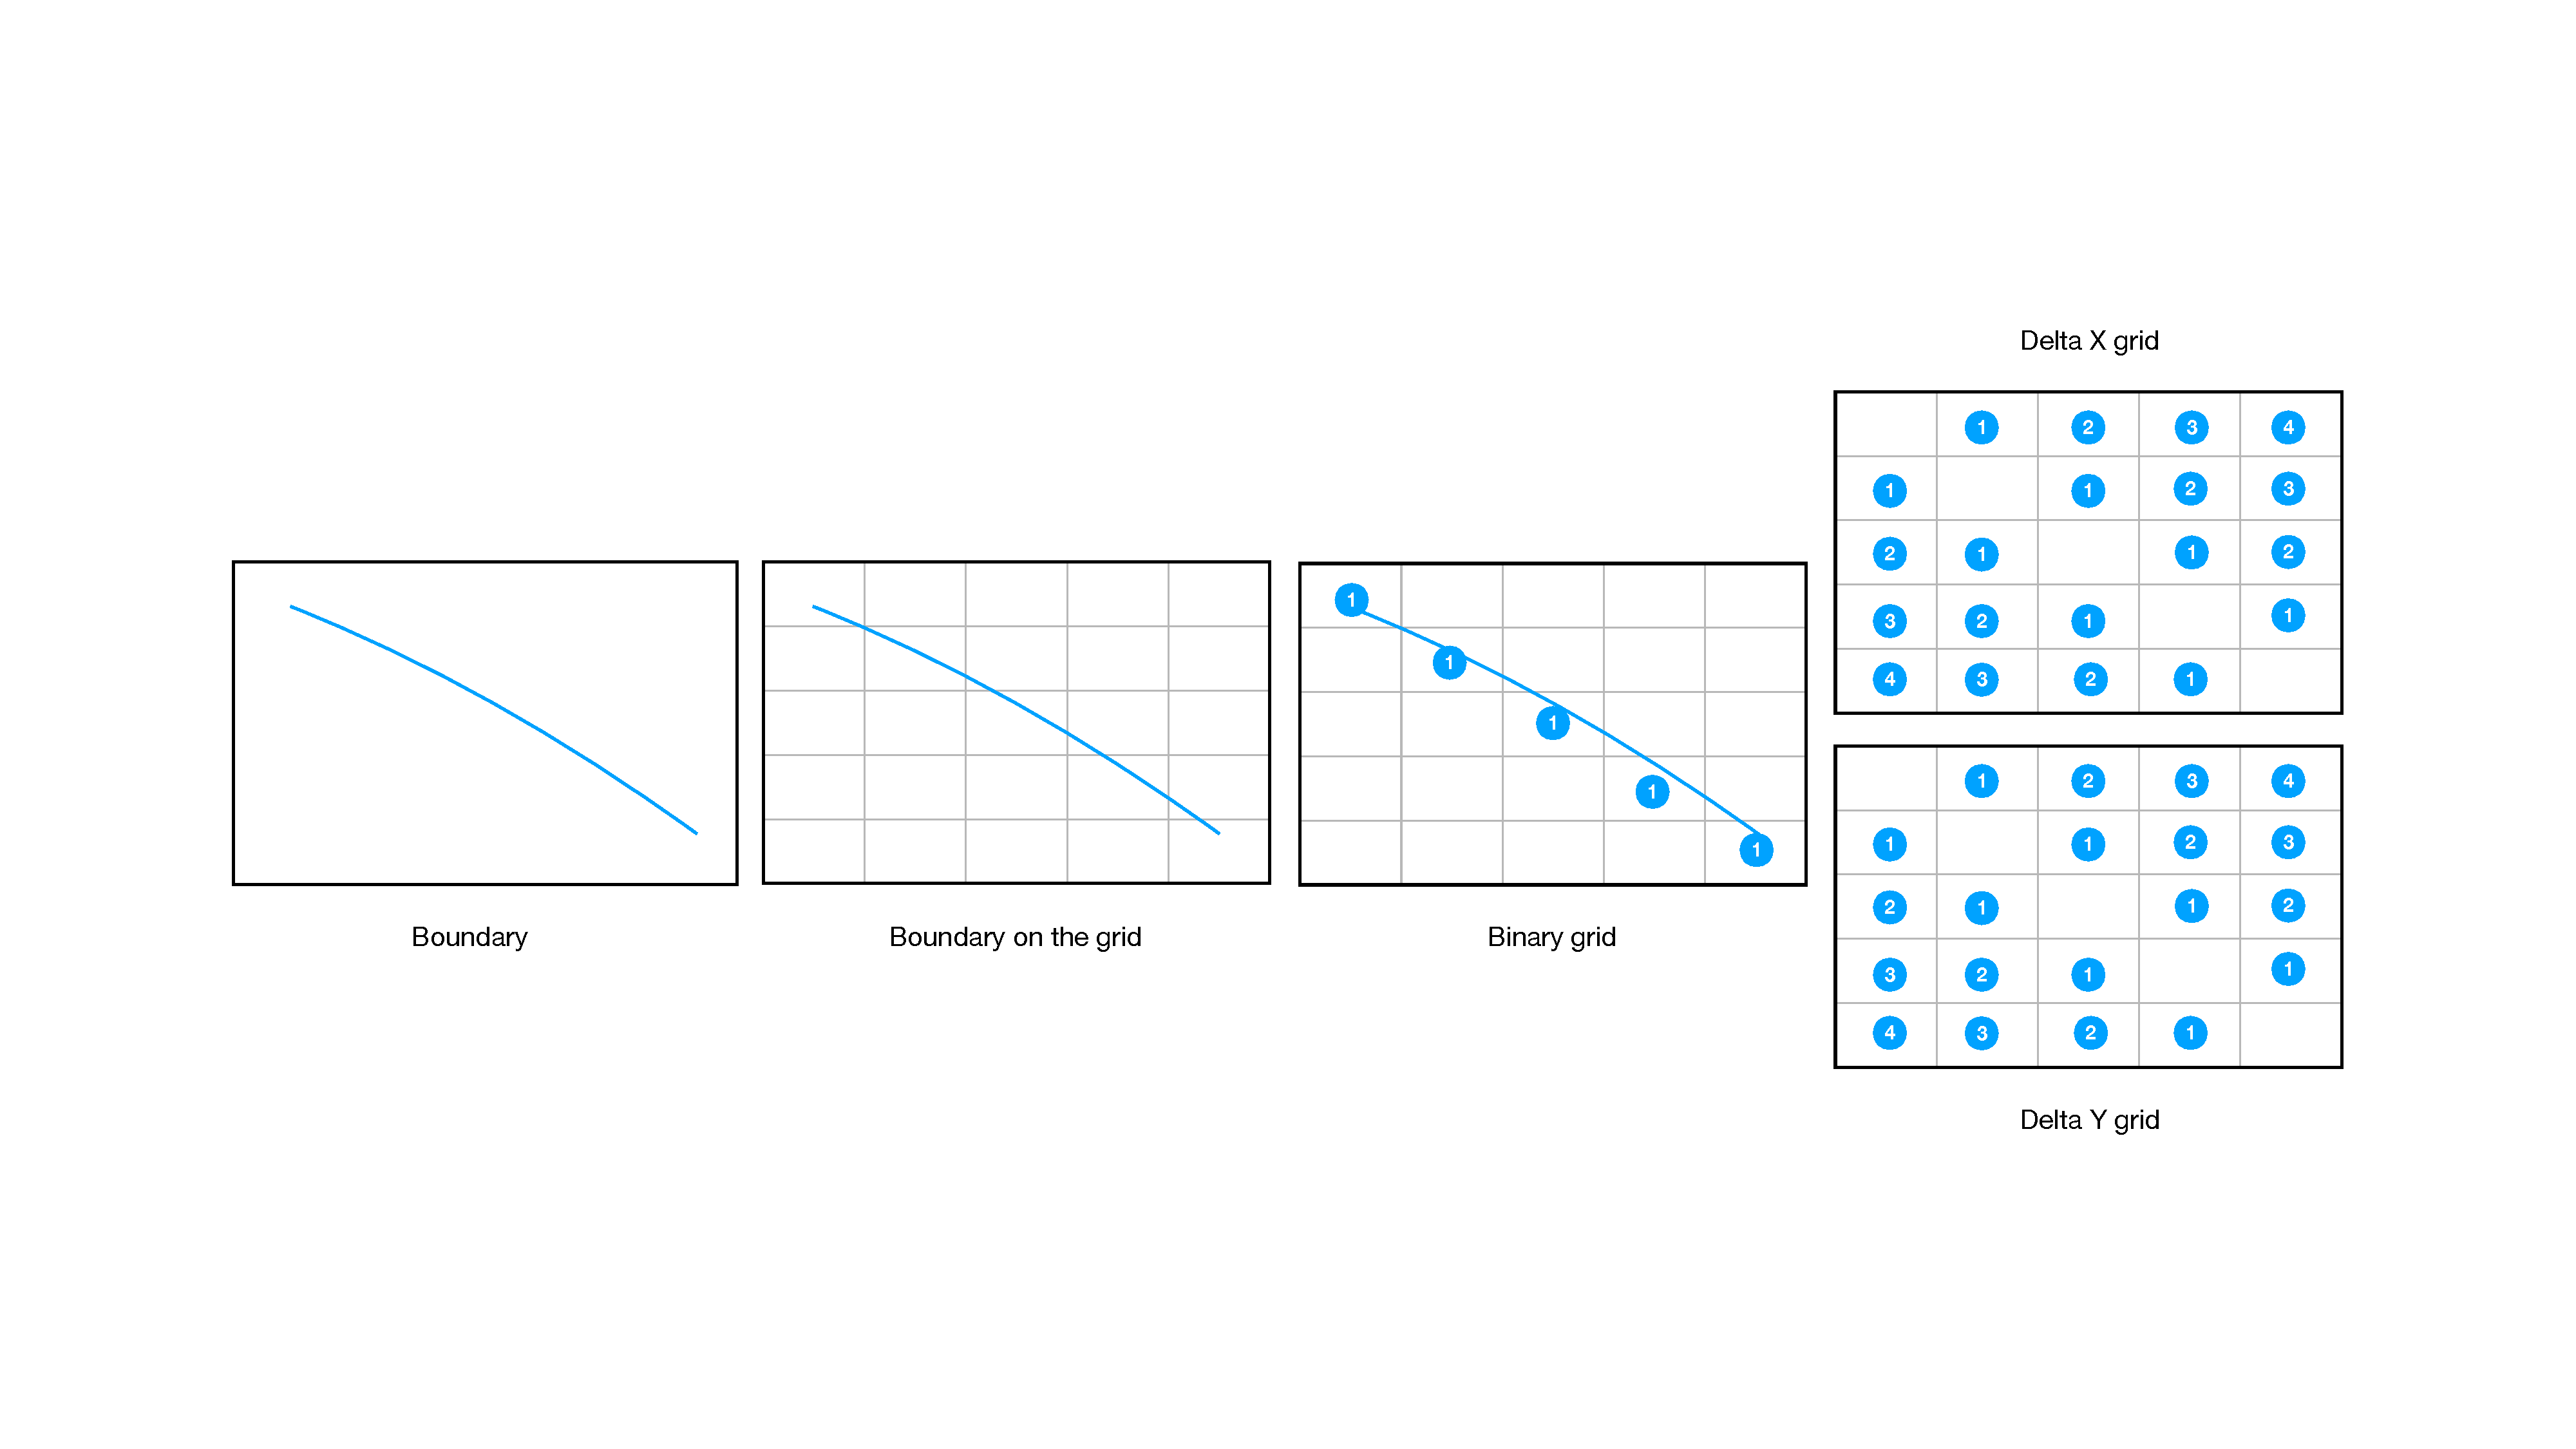
\includegraphics[width=1\linewidth]{LateX//figs/GRID.pdf}
    \caption{Proposed refinement of the grid by adding delta channels to enhance spatial encoding.}
    \label{fig:grid}
\end{figure}

This enhancement involves adding two extra channels to the boundary input tensor. These channels would encode the precise delta values from each pixel to the nearest boundary, with one channel representing the x-coordinate delta and the other the y-coordinate delta. This approach could significantly improve the model’s boundary detection capabilities by providing explicit spatial information.

Such a change enhances the model's spatial awareness, enabling it to better understand the geometric relationships within the data. The delta channels effectively act as positional encodings, allowing the model to differentiate between pixels near boundaries and those farther away. This added contextual information would likely result in more accurate predictions, particularly in scenarios with complex boundary details.

However, implementing this approach requires careful consideration:
\begin{itemize}
    \item Model Complexity: Adding these channels increases the input dimensionality, necessitating adjustments to the model architecture.
    \item Data Representation: The delta values must accurately represent the shortest distance to the boundary. Euclidean distances may be more effective than separate $x$ and $y$ deltas in some cases.
    \item Computational Efficiency: Computing delta values for each pixel could introduce additional overhead, requiring optimization to maintain efficiency.
\end{itemize} 

Another fundamental improvement involves increasing the diversity of the training dataset. The current dataset is geographically limited, as all sequences were captured in the same city along just three different roads. Expanding the dataset to include sequences from multiple cities and varied environments would enhance the network's ability to generalize to new scenarios. Exposure to different road conditions, traffic patterns, and lighting situations would help the model learn more robust features and reduce its dependency on specific geographic contexts.

Such a diverse dataset would improve the model's performance and applicability across a broader range of real-world scenarios, enhancing its robustness and reducing \textit{overfitting} risks. Furthermore, this more complex data exposure could enable the network to handle challenging conditions more effectively, such as unusual road geometries or variable environmental factors.

Another improvement could involve optimizing the sensor suite used in the current implementation. The existing setup, which relies on ten stereo cameras, is both expensive and difficult to implement in practical scenarios. Reducing the reliance on such an extensive array of sensors could make the architecture more feasible for real-world deployment while maintaining its performance for bird’s-eye view (BEV) reconstruction.

Another possible approach would be to adapt the architecture to work with mono cameras instead of stereo cameras. Mono cameras are more cost-effective and widely available, and advancements in depth estimation techniques could allow the system to approximate the depth information required for BEV reconstruction. Alternatively, the sensor setup could be simplified by using fewer sensors, such as four short-range cameras and a single central front-facing camera. This configuration would reduce redundancy while still providing sufficient coverage for BEV generation.

Future work should investigate these alternative configurations to evaluate their impact on system performance. This could include:
\begin{itemize}
    \item Investigating how mono camera setups influence the quality of depth estimation and BEV reconstruction.
    \item Evaluating the performance trade-offs when reducing the number of sensors and identifying the minimum sensor configuration required for reliable results.
    \item Exploring sensor fusion techniques to compensate for the reduced number of inputs while maintaining or improving alignment accuracy.
\end{itemize}

Reducing the complexity of the sensor suite would not only lower costs but also make the system more accessible for a wider range of applications, including lower-cost autonomous vehicles and real-time localization systems. Additionally, such an improvement could enhance the scalability of the architecture, allowing it to be deployed in diverse environments and use cases without significant hardware and calibration requirements.

In conclusion, refining the grid representation with additional spatial information and expanding dataset diversity represent critical avenues for future research. These developments have the potential to significantly improve the model’s precision, robustness, and generalizability, paving the way for more reliable applications in autonomous vehicle localization and HD map generation.